\documentclass[../main.tex]{subfiles}

\begin{document}
\providecommand{\cisco}{\lstinline{Cisco-Li 82:b2:55 (00:0c:41:82:b2:55)}}
\providecommand{\apple}{\lstinline{Apple-82:36:3a}}
\section*{L4N1 Part 2}\addcontentsline{toc}{section}{L4N1 Part 2}
\subsubsection*{Beacon Frame}
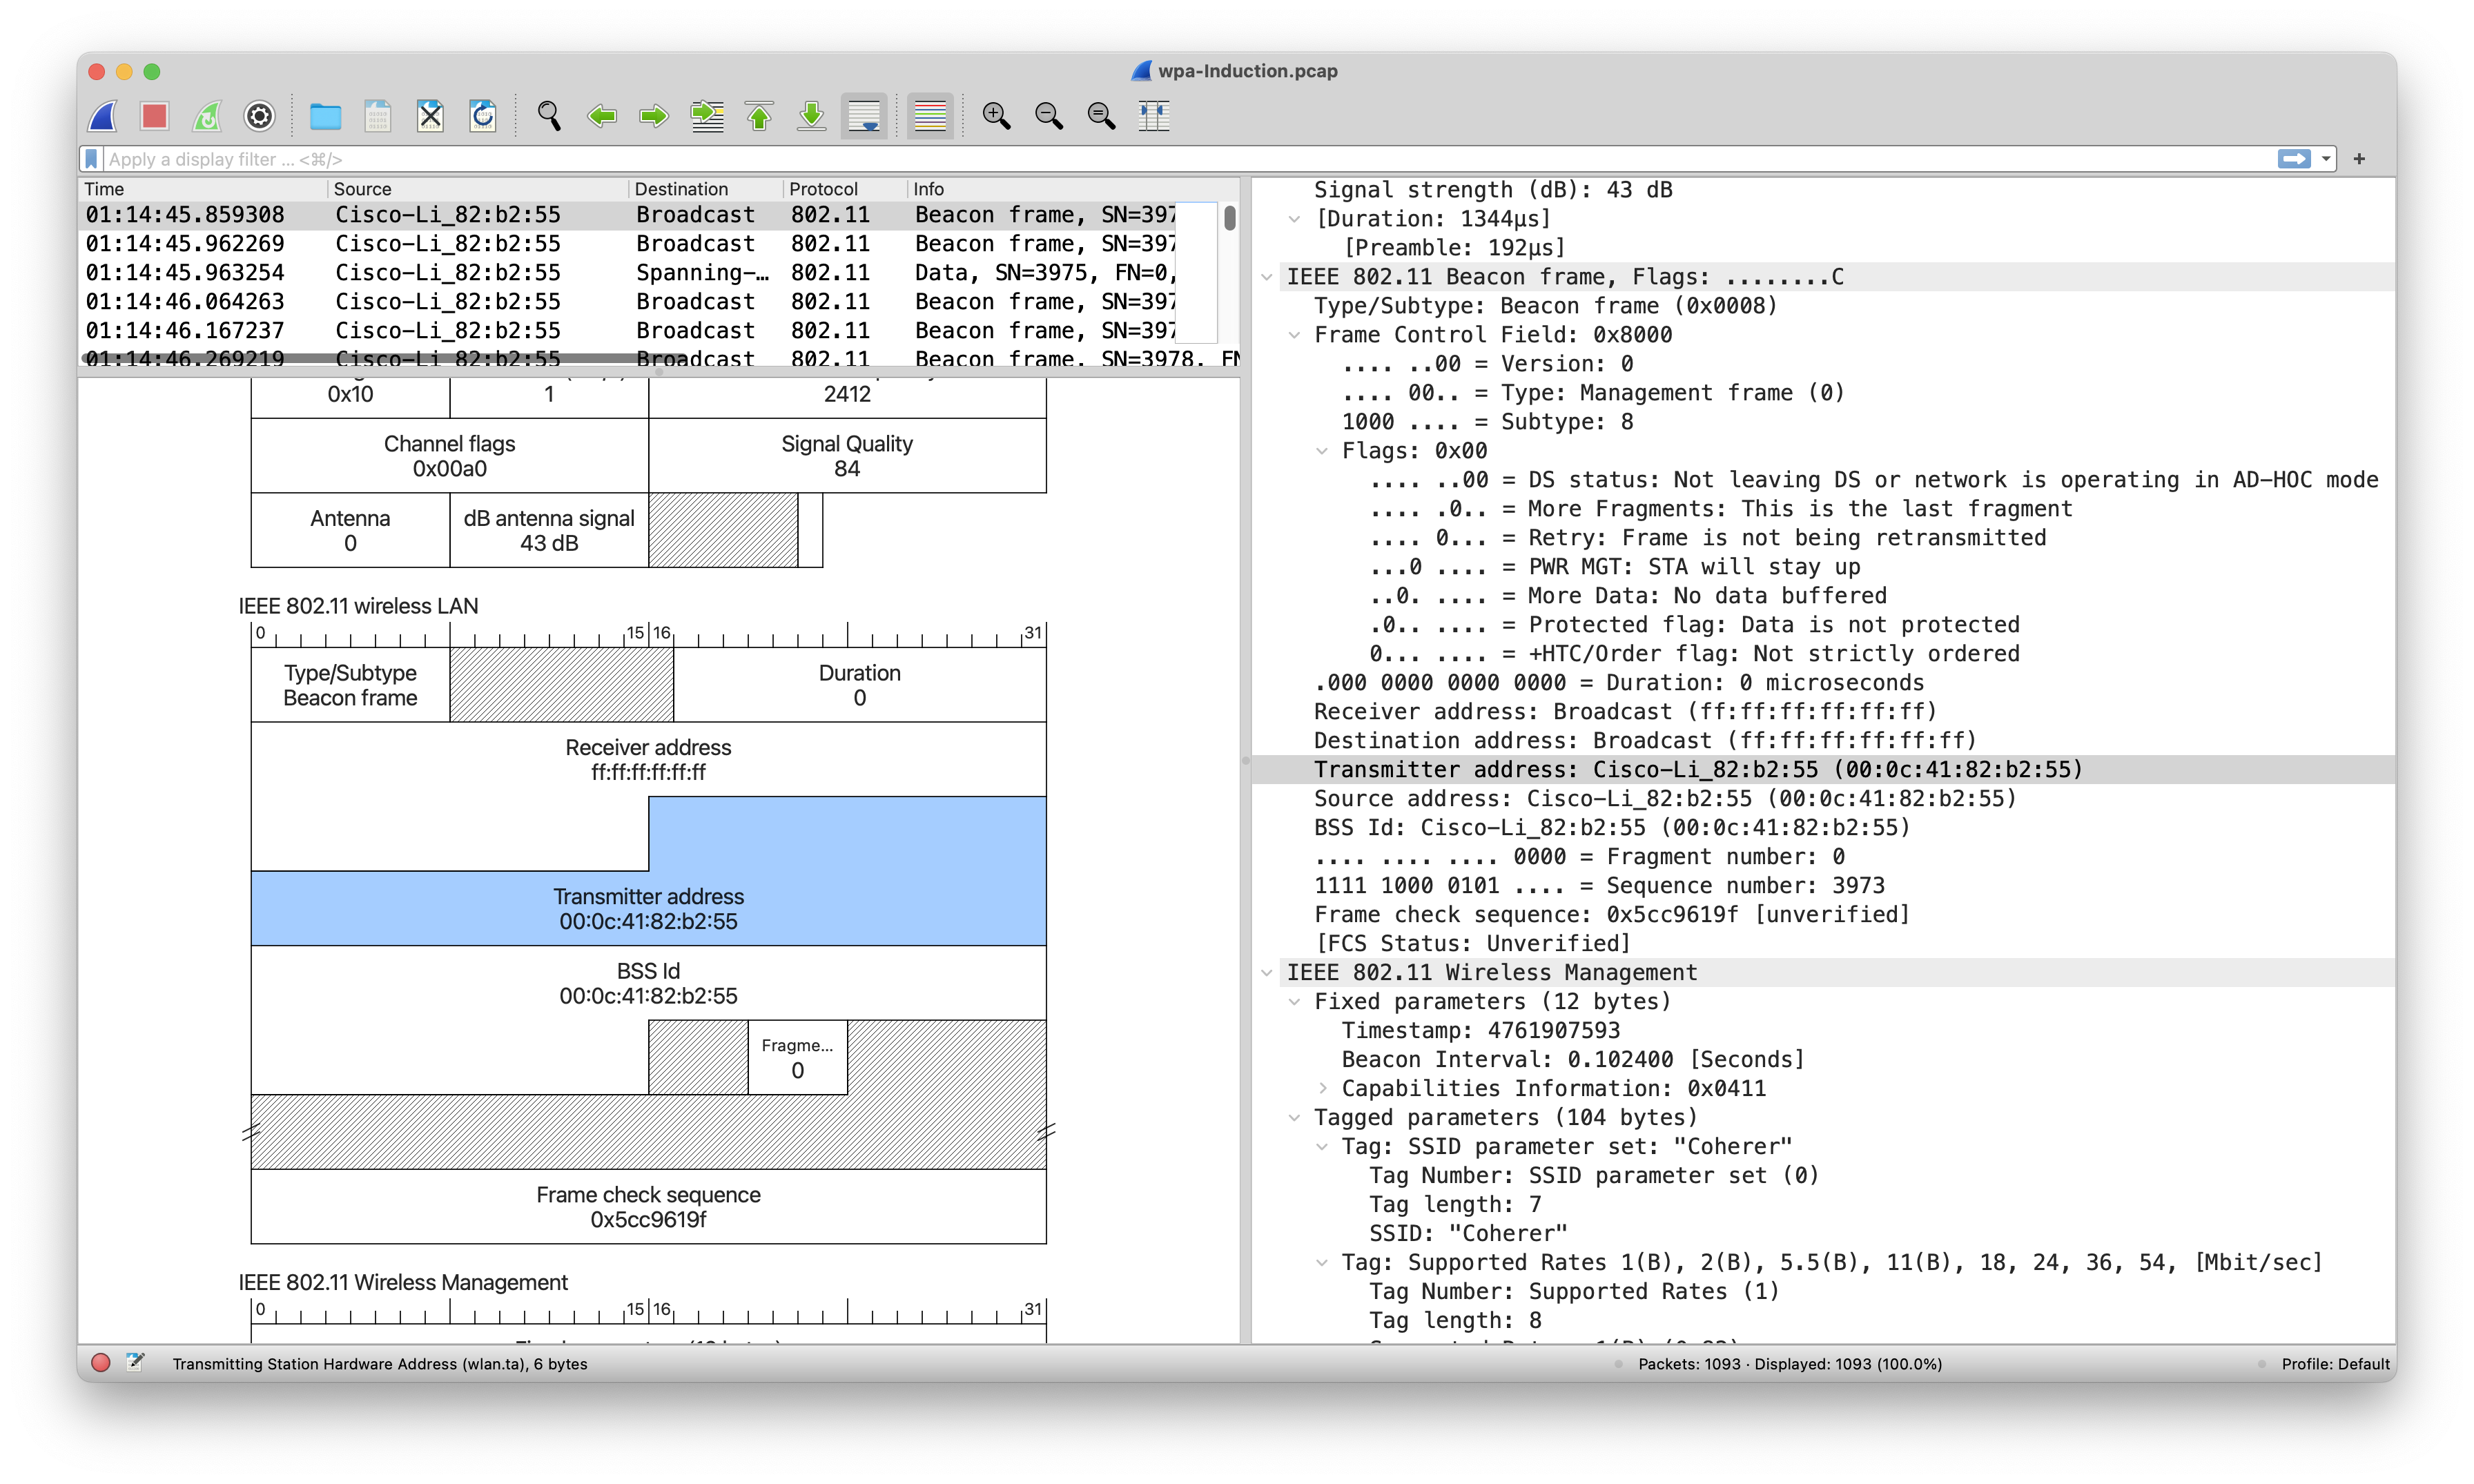
\includegraphics[width=\textwidth]{subfiles/images/PART2_Beacon_Frame.png}
\newpage

\problem{1}
\begin{wts}
    What is the SSID of the access point that is issuing the beacon frame?
\end{wts}
\begin{proof}
Consider the following excerpt of the Beacon Frame.\\
    \code{SSID = Coherer}
\end{proof}
\newpage

\problem{2}
\begin{wts}
    What are the time intervals between transmissions of beacon frames? Does the beacon frame contain this information?
\end{wts}
\begin{proof}
Consider the following excerpt of the Beacon Frame.
    \begin{lstlisting}
        IEEE 802.11 Wireless Management
        Fixed parameters (12 bytes)
        Timestamp: 4761907593
        Beacon Interval: 0.102400 [Seconds]
        Capabilities Information: 0x0411
    \end{lstlisting}
\end{proof}
\newpage

\problem{3}
\begin{wts}
    What is the source MAC address in the beacon frame?
\end{wts}
\begin{proof}
Consider the following excerpt of the Beacon Frame.\\
    \code{Transmitter address: Cisco-Li\textunderscore 82:b2:55 (00:0c:41:82:b2:55)}
\end{proof}
\newpage

\problem{4}
\begin{wts}
   What is the destination MAC address in the beacon frame? What does this address mean?
\end{wts}
\begin{proof}
Consider the following excerpt of the Beacon Frame.\\
    \code{Destination address: Broadcast (ff:ff:ff:ff:ff:ff)}
\end{proof}
\newpage

\problem{5}
\begin{wts}
   How many data rates can the access point support?
\end{wts}
\begin{proof}
Consider the following excerpt of the Beacon Frame.
    \begin{lstlisting}
        Tag: Supported Rates 1(B), 2(B), 5.5(B), 11(B), 18, 24, 36, 54, [Mbit/sec]
        Tag Number: Supported Rates (1)
        Tag length: 8
        Supported Rates: 1(B) (0x82)
        Supported Rates: 2(B) (0x84)
        Supported Rates: 5.5(B) (0x8b)
        Supported Rates: 11(B) (0x96)
        Supported Rates: 18 (0x24)
        Supported Rates: 24 (0x30)
        Supported Rates: 36 (0x48)
        Supported Rates: 54 (0x6c)\end{lstlisting}
\end{proof}
\newpage

\problem{6}
\begin{wts}
   Examine the beacon frame, what frequency does the advertised network use?
\end{wts}
\begin{proof}
Consider the following excerpt of the Beacon Frame.
    \begin{lstlisting}
        802.11 radio information
        PHY type: 802.11b (HR/DSSS) (4)
        Short preamble: False
        Data rate: 1.0 Mb/s
        Channel: 1
        Frequency: 2412MHz
        Signal strength (dB): 43 dB
        [Duration: 1344\mu s]
        [Preamble: 192\mu s]\end{lstlisting}
\end{proof}
\newpage

\problem{7}
\begin{wts}
    By looking at the list plane, indicate what type of packets have the smallest size? What type has the largest size?
\end{wts}
\begin{proof}
    We will refrain from using the term packet, as the discussion that subsequently follows involve solely link-layer communications. And will use the term 'packet' only in the internetworking context. From the list of frames obtained in the trace, it is clear that Acknowledgement, and 'Clear-to-Send' frames have the smallest size. Consider the following excerpt from the trace.\\
    \begin{lstlisting}
        01:14:47.468019		Cisco-Li_82:b2:55 (00:0c:41:82:b2:55) (RA)	802.11	38	Acknowledgement, Flags=........C\end{lstlisting}
    and
    \begin{lstlisting}
        01:14:51.508269		Cisco-Li_82:b2:55 (00:0c:41:82:b2:55) (RA)	802.11	38	Clear-to-send, Flags=........C\end{lstlisting}
    Data frames have the largest size, capped at $1576$
    \begin{lstlisting}
        01:15:12.724726	Cisco-Li_82:b2:53	Apple_82:36:3a	802.11	1576	Data, SN=302, FN=0, Flags=.p....F.C\end{lstlisting}
\end{proof}
\newpage


\problem{8}
\begin{wts}
    Before sending data to \lstinline{Apple_82:36:3a}, what frames are exchanged between this device and the access point?
\end{wts}
\begin{proof}
    The frames exchagned are, prior to data transfer,m
    \begin{itemize}
        \item Probe request,
        \item Probe response,
        \item Acknowledgement,
        \item Authentication,
        \item Association request,
        \item Key,
        \item Clear-to-send,
        \item Beacon Frame
    \end{itemize}
\end{proof}
\newpage


\problem{9}
\begin{wts}
    Examine the Authentication frame sent by \lstinline{Apple_82:36:3a}, does the host want the authentication to require a key or be open?
\end{wts}
\begin{proof}
    Consider the following excerpt from the Authentication Frame sent by \apple.
    \begin{lstlisting}
        IEEE 802.11 Wireless Management
        Fixed parameters (6 bytes)
        Authentication Algorithm: Open System (0)
        Authentication SEQ: 0x0001
        Status code: Successful (0x0000)
    \end{lstlisting}
    It is clear that the host wants\\
    \lstinline{Authentication Algorithm: Open System (0)}
\end{proof}
\newpage

\problem{10}
\begin{wts}
    Examine the response Authentication frame sent by the AP to \apple. What is the Association ID for this host? What is the usage of this ID?
\end{wts}
\begin{proof}
    See Problem 9, the Association ID for the host is\\
    \lstinline{Authentication SEQ: 0x0001}\\
    The Wireshark Info reads,
    \begin{lstlisting}
        Authentication Sequence Number (wlan.fixed.auth_seq), 2 bytes
    \end{lstlisting}
    The response form \cisco to \apple is another frae with \\
    \lstinline{Authentication SEQ: 0x0002}\\
    acknowledges the authentication attempt by the end-system \apple.
\end{proof}
\newpage

\problem{11}
\begin{wts}
    What transmission rates is the host willing to use? The AP? To answer this question, you will need to look into the parameters fields of the 802.11 wireless LAN management frame.
\end{wts}
\begin{proof}
    Consider the following graphics.\\
    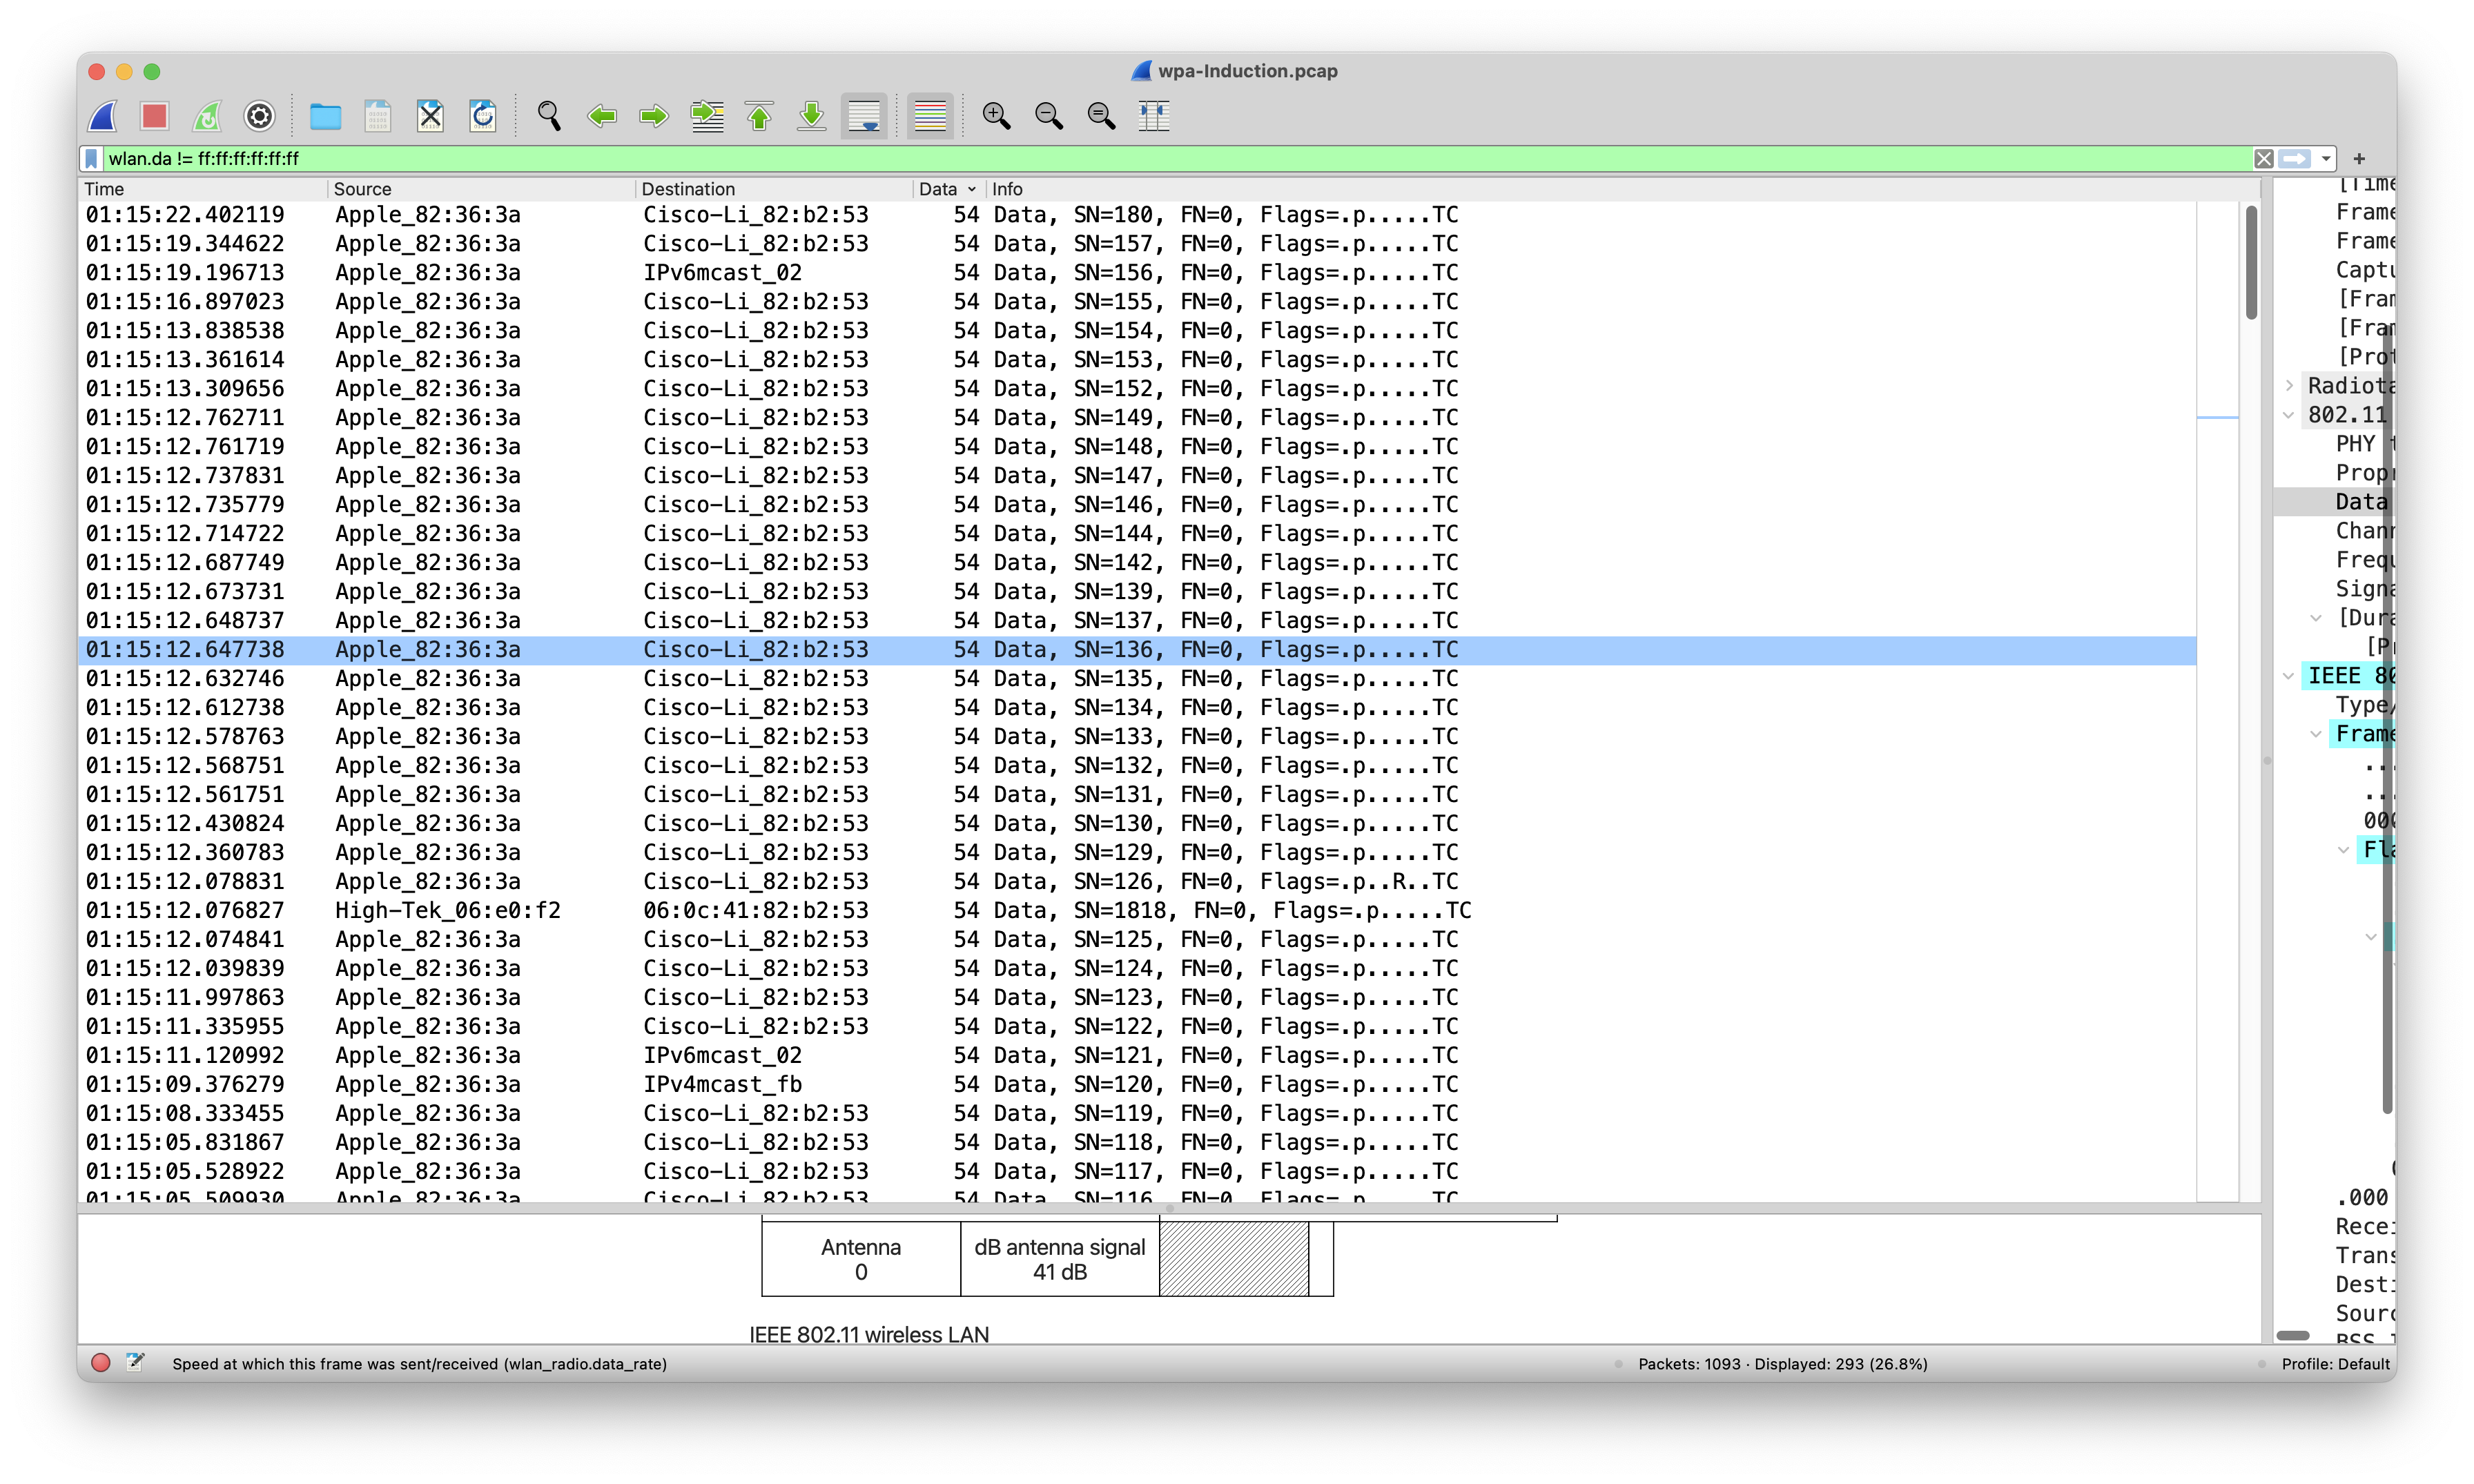
\includegraphics[width=\textwidth]{subfiles/images/PART2_Q11_RATES_1.png}
    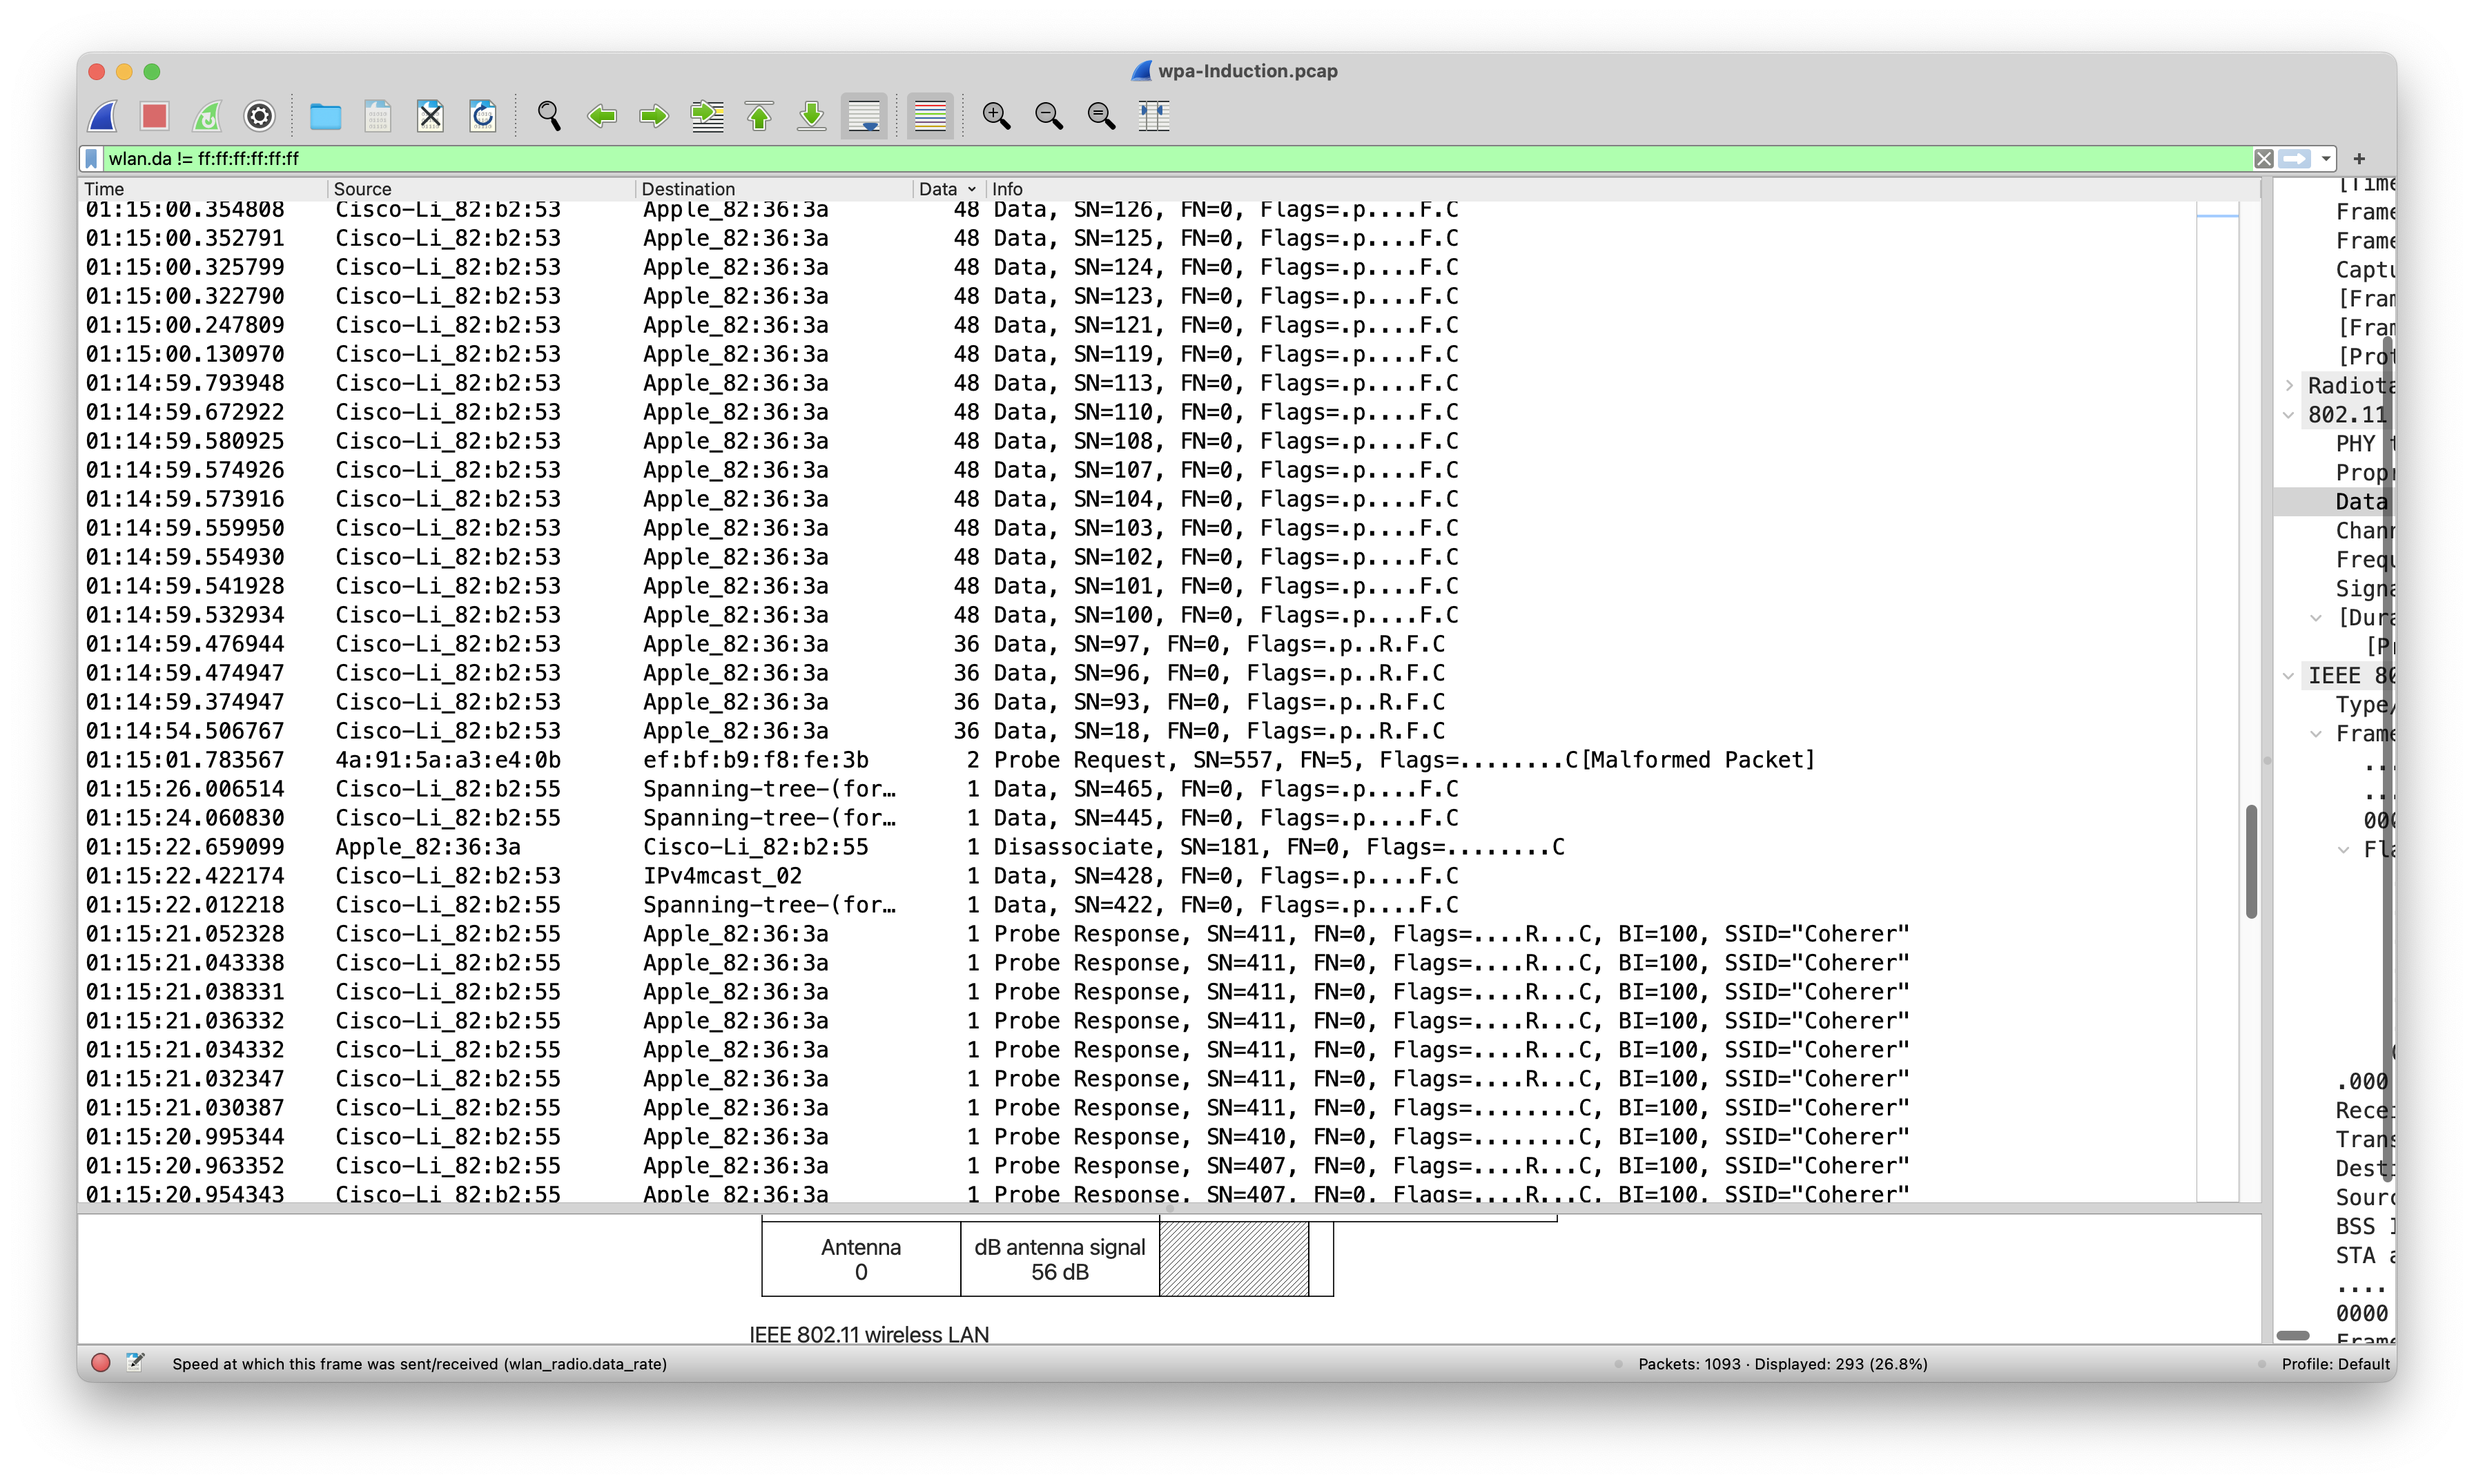
\includegraphics[width=\textwidth]{subfiles/images/PART2_Q11_RATES_2.png}
    It is clear that \apple transmits at $1$ or $54$ Mbps, while \cisco transmits at $1$, $36$, $48$, or $54$ Mbps.
\end{proof}
\newpage

\problem{12}
\begin{wts}
    Examine the Disassociation frame sent by \apple to the \cisco. What is the reason that this user sent Disassociation frame?
\end{wts}
\begin{proof}
    Consider the following excerpt from the Disassociation Frame,\\
    \begin{lstlisting}
        IEEE 802.11 Wireless Management
        Fixed parameters (2 bytes)
        Reason code: Disassociated because sending STA is leaving (or has left) BSS (0x0008)\end{lstlisting}
\end{proof}

\end{document}